% Section: Constraint Composition (compressed, 787→~500 words)

% ──────────────────────────────────────────
%  Figure: Composition Interaction
% ──────────────────────────────────────────
\begin{figure}[t]
\centering
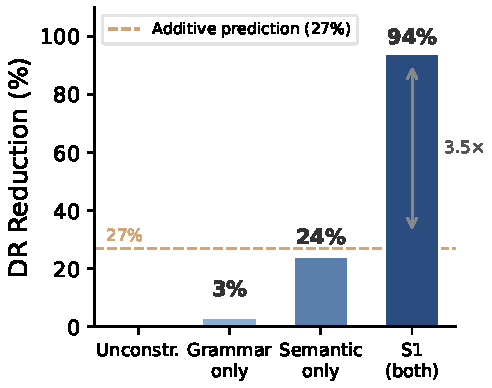
\includegraphics[width=\columnwidth]{figures/fig_composition_interaction.pdf}
\caption{Non-additive layer interaction on SciERC (Qwen3-8B, zero-shot). Grammar-only and semantic-only achieve 3\% and 24\% DR reduction; their composition yields 94\%, 3.5$\times$ the additive prediction.}
\label{fig:composition-interaction}
\end{figure}

At each decoding step $t$, let $G(t) \subseteq V$ and $S(t) \subseteq V$ denote the tokens permitted by the grammar and semantic layers, respectively.
The final mask is their conjunction:
%
\begin{equation}\label{eq:composition}
  M_{\text{final}}(t) = M_{\text{grammar}}(t) \;\wedge\; M_{\text{semantic}}(t),
\end{equation}
%
where $\wedge$ denotes element-wise AND over the vocabulary $V$; a token is allowed only if it satisfies \emph{both} structural and type-level constraints.
The conjunction is asymmetric: $S(t)$ is defined only over $G(t)$. This reflects the scale-dependent layer interaction (\S\ref{sec:method}): the semantic layer requires the relation type to belong to $\mathcal{R}$, a property enforced only by the grammar layer.
This dependency is scale-sensitive: 70B semantic-only achieves 84\% DR reduction (vs.\ 24\% on 8B), though grammar remains necessary for RV elimination (\S\ref{sec:70b-results}).

\paragraph{Grammar-First Fallback.}
When $S(t) \cap G(t) = \emptyset$ (tight constraints leave no token that is both grammar-valid and semantically valid), na\"{\i}ve masking would force selection of a grammar-invalid token, breaking JSON structure.
We enforce a \emph{grammar-first fallback}: semantic masking is skipped and the grammar layer alone controls selection.
Structural integrity is a hard constraint; type violations are soft errors detectable by downstream validation, with DR (ontologically invalid type pair) more severe than CF (individually valid triples with cross-triple type inconsistency).
Extraction tasks are robust to format-level constraints~\cite{tam2024letmespeak}, supporting this asymmetric treatment.

\paragraph{Constraint Tightness.}
\label{eq:tightness}
Per-relation constraint tightness $\kappa(r) = 1 - |\sigma(r)|/|\mathcal{E}|^2$ captures schema restrictiveness; DR reduction correlates descriptively with schema-mean $\bar{\kappa}$ across our three evaluation schemas ($n{=}3$), though entity type confusability is a significant co-factor (Appendices~\ref{app:kappa-case-study},~\ref{app:kappa-analysis},~\ref{app:tcr}).
Figure~\ref{fig:dual-factor-scatter} shows that residual DR is governed by the product $\bar{\kappa} \times \text{RV}_{\text{baseline}}$ for calibrated models ($R^2{=}0.886$, $n{=}4$; descriptive only).

% ──────────────────────────────────────────
%  Figure: Dual-Factor Scatter (moved from appendix)
% ──────────────────────────────────────────
\begin{figure}[t]
\centering
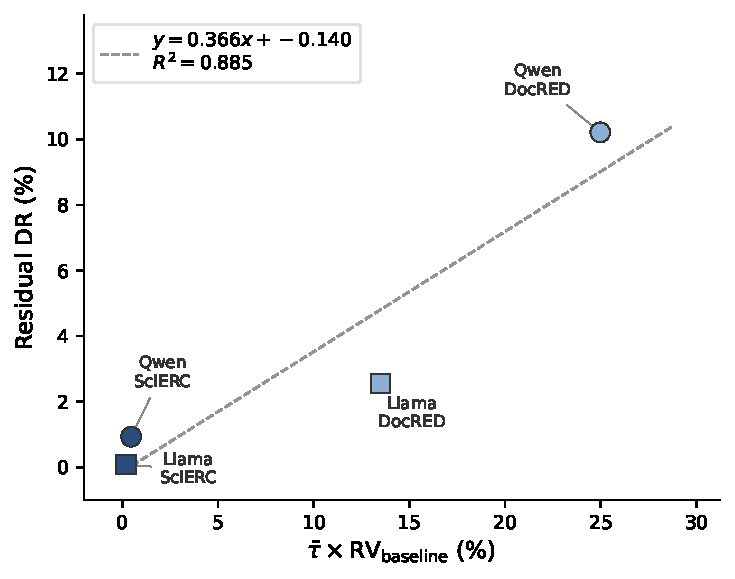
\includegraphics[width=\columnwidth]{figures/dual_factor_scatter.pdf}
\caption{Residual DR vs.\ $\bar{\kappa} \times \text{RV}_{\text{baseline}}$ across model$\times$dataset configurations. Linear fit (calibrated models): $R^2{=}0.886$ ($n{=}4$, $p{=}0.058$; descriptive only).}
\label{fig:dual-factor-scatter}
\end{figure}

\paragraph{Greedy limitation and fallback cascade.}
\label{sec:greedy-limitation}
Single-pass per-triple enforcement cannot coordinate type assignments across triples sharing the same entity mention; cross-field consistency requires global inference that exceeds the per-token masking paradigm.
The semantic layer commits entity types greedily, an instance of Level~3 (non-local) constraints (\S\ref{sec:decidability}), so CF violations arise when the same entity receives different types across triples; beam search mitigates this (\S\ref{sec:beam-results}).
Fallback triggers on 0.5--5.7\% of type-bearing positions (zero-shot), virtually eliminated by fine-tuning ($\leq$\,0.11\%); all residual DR occurs at fallback positions (Appendices~\ref{app:causal-tracing},~\ref{app:fallback-coverage}).

\paragraph{Non-rectangularity and independent enforcement.}
\label{sec:rectangularity}
Type signatures are non-rectangular (0/7 SciERC, 23/96 DocRED rectangular); independent enforcement admits 33--37\% spurious pairs, eliminated by fine-tuning (Table~\ref{tab:composability}).
Shuffling type order produces byte-identical outputs across all 551 SciERC documents, confirming order invariance (Appendix~\ref{app:order-invariance}).

